\begin{tikzpicture}[
    stage label/.style={anchor=west},
    image/.style={box, text width=, rounded corners, inner sep=0pt}
]
    \node(n0){Input Data};
    \node[image, right=of n0](n1){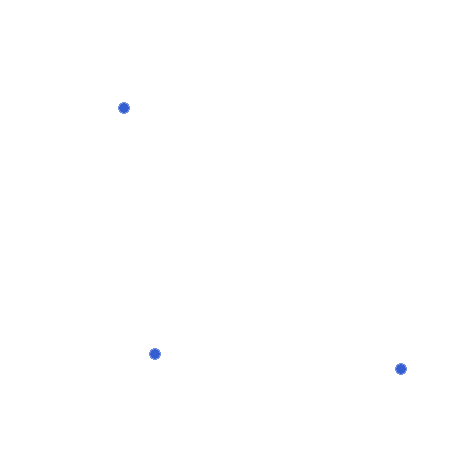
\includegraphics[width=100pt]{figures/VertexShaderStage.png}};
    \node[image, right=of n1](n2){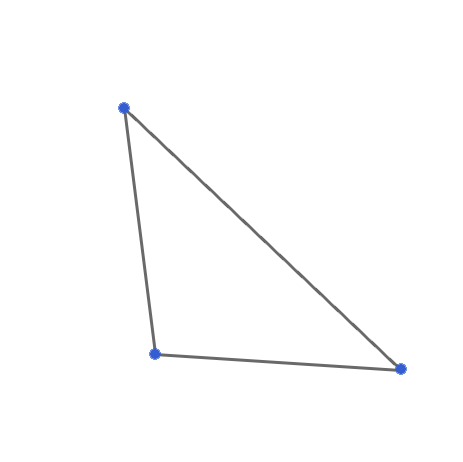
\includegraphics[width=100pt]{figures/VerticesAndEdges.png}};
    \node[image, below=of n2](n3){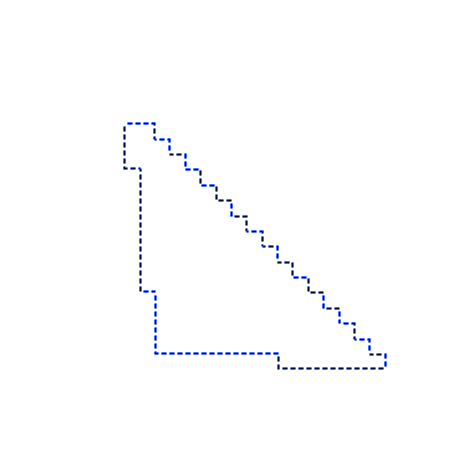
\includegraphics[width=100pt]{figures/Rasterized.png}};
    \node[image, left=of n3](n4){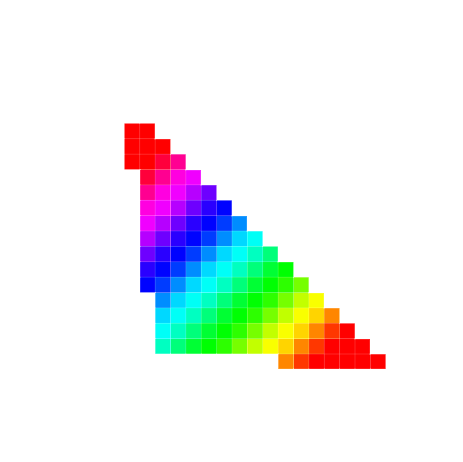
\includegraphics[width=100pt]{figures/FragmentShader.png}};
    \node[left=of n4](n5){Framebuffer};

    \draw[arrow](n0) -- node[stage label,rotate=90]{Vertex Shader} (n1);
    \draw[arrow](n1) -- node[stage label,rotate=90]{Triangle Assembly} (n2);
    \draw[arrow](n2) -- node[stage label]{Rasterization} (n3);
    \draw[arrow](n3) -- node[stage label,rotate=90]{Fragment Shader} (n4);
    \draw[arrow](n4) -- node[stage label,rotate=90]{Blend} (n5);
\end{tikzpicture}